\section{Anwendung der Methodik auf die theoretischen Grundlagen}

\subsection{Prototypische Implementierung der Integrations- und Bereitstellungs-Pipelines}
\subsection{Evaluation der Integrations- und Bereitstellungs-Pipelines unter Anwendung des Analytischen Hierarchieprozesses}
\label{sec:AHP}
Als Entscheidungsalternativen werden CI/CD-Pipelines für die Bereitstellung von Cloud-Software gegenübergestellt. Konkret handelt es sich dabei, um die Tools \textit{SAP CI/CD}, \textit{Jenkins}, sowie \textit{Azure Pipelines}. Die Gegenüberstellung wird auf die genannten CI/CD-Pipelines beschränkt, da ausschließlich diese von der SAP vorgeschlagen werden. Bei der Untersuchung der Pipelines sind dabei verschiedene Aspekte zu beachten. So soll im Rahmen der Arbeit evaluiert werden, ob sich die verschiedenen Pipelines zur Bereitstellung von Software für CEs eignet. Weiterhin muss festgestellt werden, inwiefern die Tools für die Technologien SAP CAP bzw. SAP UI5 geeignet sind und ob eine Bereitstellung in der Laufzeitumgebung Cloud Foundry der SAP BTP möglich ist. 
\subsubsection{Festlegung der hierarchischen Entscheidungskriterien}
 Die zur Durchführung des AHP-Verfahrens benötigten Daten werden neben einer Literaturrecherche ebenfalls mittels Experteninterviews erhoben. Für die Experteninterviews wird eine Expertengruppe aus 6 Mitarbeitenden der SAP zusammengestellt. Diese sind jeweils in verschiedenen Bereichen der Cloud-Fullstack-Entwicklung, Test-Management, sowie im DevOps spezialisiert. Somit kann Expertise über verschiedene Fachbereiche hinweg aufgebaut und Anforderungen aller an der Entwicklung, Bereitstellung sowie an dem Betrieb von Software beteiligten Stakeholdern erfasst werden. Zur Festlegung der Entscheidungskriterien wird eine induktive Kodierung der Expertengespräche durchgeführt (s. Anhang \ref{sec:kodierung}). Dabei werden aus besonders häufig von Experten genannten Aspekten systematisch Kategorien abgeleitet. Diese umfassen insbesondere Aspekte, welche die in vergangenen Kundenprojekten hervorgegangenen Anforderungen an eine CI/CD-Pipeline widerspiegeln. Da innerhalb dieser Kundenprojekte oft weniger strikte Qualitätsanforderungen an den CI/CD-Prozess gestellt werden, wird darüber hinaus erarbeitet, welche internen Bestimmungen von der SAP zur Bereitstellung von Standardsoftware definiert werden. Die bei der induktiven Kodierung erhobenen Kategorien werden anschließend ebenfalls als Entscheidungskriterien im AHP-Verfahren wiederverwendet. Die mit dieser Vorgehensweise erhobenen Entscheidungsalternativen sind folgender Abbildung zu entnehmen:
 \begin{center}
	\begin{figure}[H]
		\centering
		\scalebox{0.5}{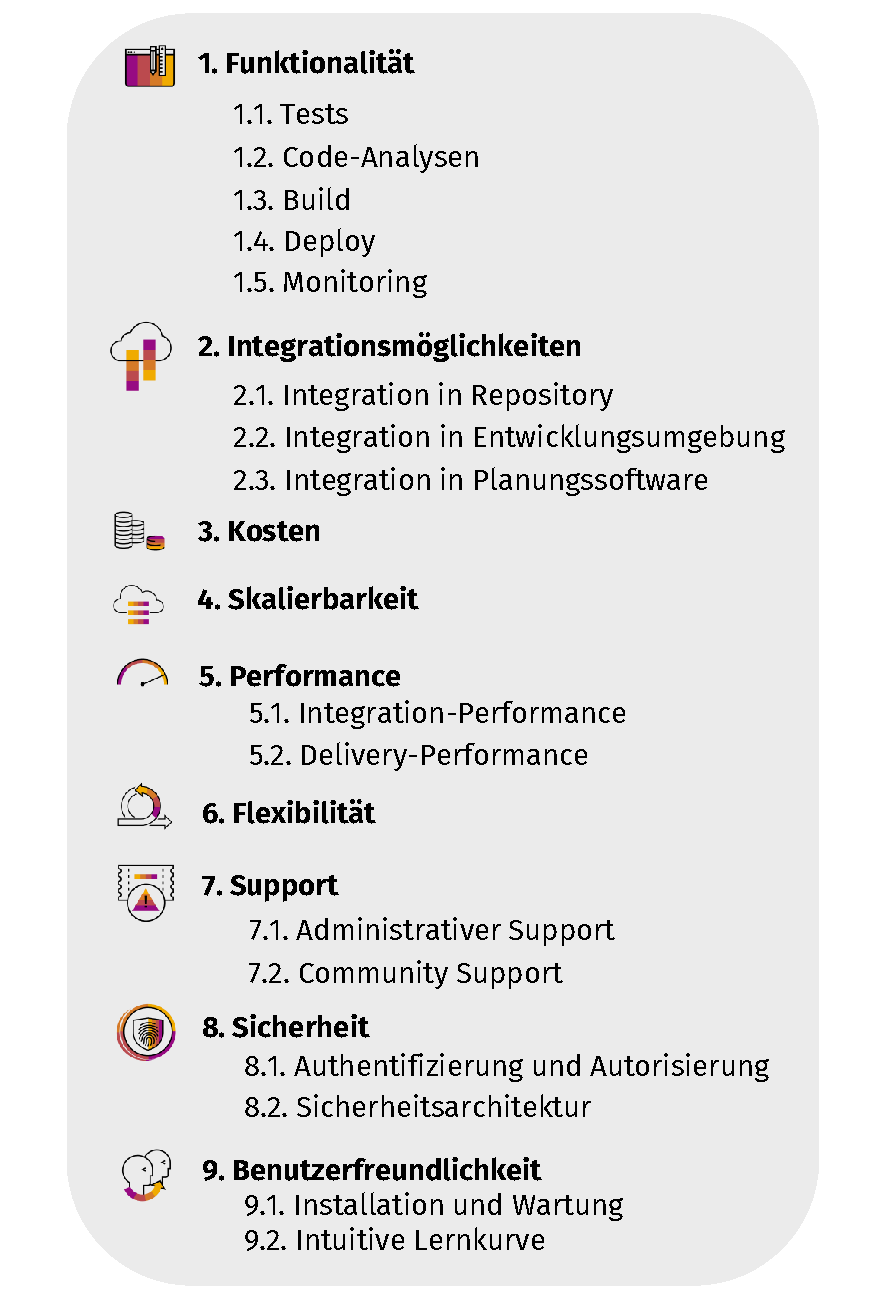
\includegraphics{AHP_E}}
		\caption[AHP-Entscheidungsstruktur zur Bewertung von CI/CD-Pipelines]{AHP-Entscheidungsstruktur zur Bewertung von CI/CD-Pipelines. Eigene Darstellung.}
		\label{fig:AHP_E}
	\end{figure}
\end{center}
\vspace*{-15mm}
 Auf der obersten Ebene des AHP-Entscheidungsbaums werden neun Kategorien definiert. Das erste Kriterium ist \textbf{Funktionalität} (K1). Diese Kategorie umfasst verschiedene innerhalb des CI/CD-Workflows benötigte funktionale Spezifikationen. So sollte eine Pipeline etwa dazu in der Lage sein, Anwendungen zu testen, Code-Analysen durchzuführen und eine Software auf der Cloud-Plattform bereitzustellen. Experte 1 begründet dabei, dass es \enquote{eine Unterstützung dieser Stufen benötigt, um eine effiziente Bereitstellung von Software zu ermöglichen} \cite[Z. 52]{ProductOwnerSAPBTPProd&Infra.}.  Angesichts der Vielfältigkeit des Entscheidungskriteriums Funktionalität, wird eine Untergliederung in verschiedene Subkriterien vorgenommen. In Kategorie 1.1 wird evaluiert, welche Tests von der Pipeline unterstützt werden. Von der SAP werden diesbezüglich Produktstandards vorgegeben. Diese stützen sich auf \textit{ISO 9001}, eine internationale Norm für Qualitätsstandards. Im Kontext der Softwareentwicklung verlangt diese, eine für neue Funktionalitäten kontinuierliche und automatisierte durchgeführte Prüfung. Dies erfordert eine Abwicklung von Unit-, Integration-, E2E-Test sowie Manual-Tests für Backend sowie Frontend. Hinsichtlich der Entwicklung von CAP-Node-Anwendungen wird in der SAP die Durchführung von Unit-Tests mittels Jest bzw. Mocha und Integration-Tests mittels Newmann vorgeschlagen. Für die Programmierung mit SAP UI5 sind hingegen Unit-Tests mittels Q-Unit, Integration-Tests mittels OPA5 und E2E-Tests mittels WDI5 vorgesehen. Während die Test-Frameworks Jest, Mocha, Newmann sowie Q-Unit in einer herkömmlichen Node-Laufzeitumgebung ausgeführt werden, benötigt es für OPA5 sowie WDI5 einer emulierten Browser-Umgebung (Webdriver.io). Die von dem Emulator generierte Benutzeroberfläche ermöglicht das Simulieren und Testen von gezielten Anwenderinteraktionen. Diese können z.B. das Ausfüllen von Formularen bzw. das Klicken auf Schaltflächen darstellen. Bei der Bewertung soll deshalb insbesondere evaluiert werden, ob neben der Node-Laufzeitumgebung ebenfalls eine emulierte Browser-Umgebung von den zu vergleichenden Pipelines unterstützt wird.\\ 
In Kriterium K1.2 wird die Kompatibilität verschiedener \textit{Code-Analyse-Tools} untersucht. Es wurde gezielt eine Trennung dieser Kategorie mit dem Kriterium K1.2 (Tests) vorgenommen. Während Tests eine funktionale Erfüllung der Anforderung evaluieren, werden mit Code-Analysen Code-Qualitätsstandards der entwickelten Features untersucht. Dabei wird evaluiert, ob statische Codeanalysen, Security- sowie Performance-Überprüfungen von den CI/CD-Pipelines unterstützt werden. Gemäß den Produktstandards der SAP sind für statische Code-Analysen Lint sowie SonarQube vorgeschrieben. Mit diesen Tools können neben syntaktischen Formqualitätsüberprüfungen ebenfalls Code-Metriken wie Komplexität oder Quellcode-Duplikate analysiert werden. Zur Durchführung von Sicherheitsüberprüfungen wird für SAP-CAP-Node-Anwendungen Checkmarx verwendet, während für SAP UI5 DASTER zum Einsatz kommt. Während für Performance-Tests von der SAP das Tool JMeter vorgeschlagen wird, gibt es bezüglich der Code-Coverage-Checks keine spezifische Vorgabe.\\
In der Kategorie K1.3 werden die \textit{Build-Funktionalitäten} der CI/CD-Pipelines evaluiert. 
Um Anwendungen in die Cloud-Foundry-Laufzeitumgebung der SAP BTP bereitzustellen, wird i.d.R. das Mulit-Target-Application-Konzept (MTA-Konzept) verwendet.
\begin{center}
	\begin{figure}[H]
		\centering
		\scalebox{0.25}{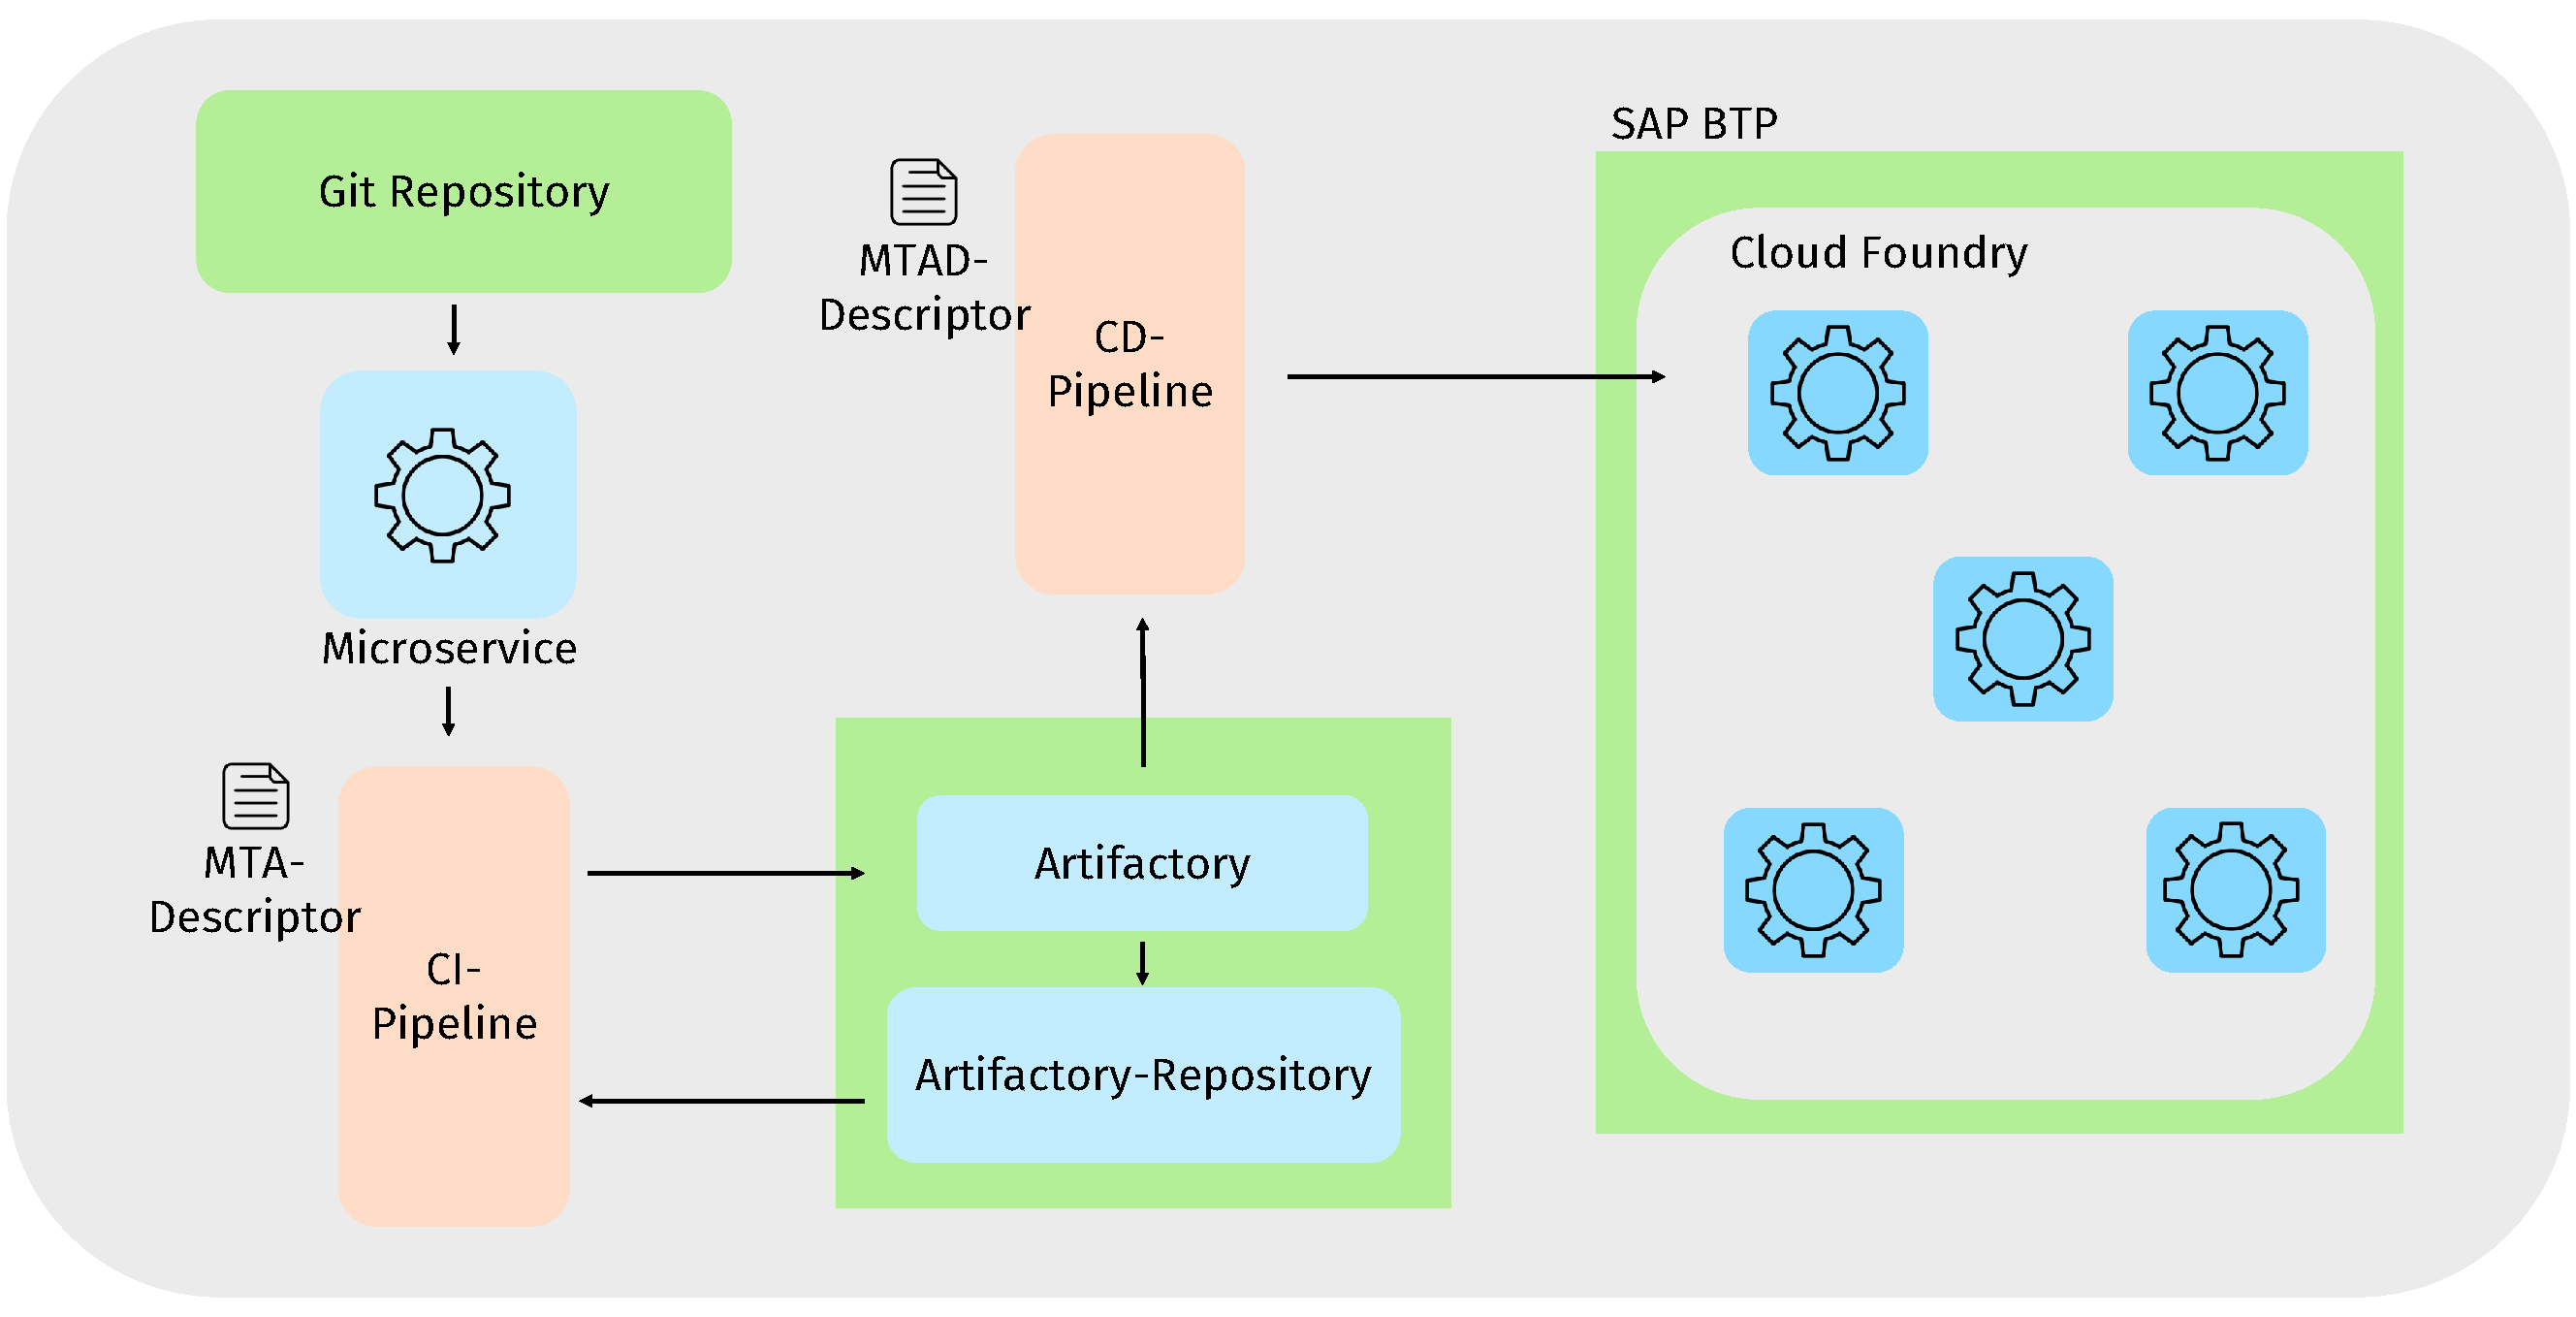
\includegraphics{MTA}}
		\caption[Bereitstellung von MTA-Applikationen in ein Artefakt-Repository]{Bereitstellung von MTA-Applikationen in ein Artefakt-Repository. Eigene Darstellung.}
		\label{fig:MTA}
	\end{figure}
\end{center}
\vspace*{-15mm}
Die MTA ist eine Applikation, z.B. ein Microservice eines CEs, welche aus verschiedenen Modulen besteht. Diese Module umfassen typischerweise die durch einen Microservice bereitgestellte API oder eine von der Applikation verwendete Datenbank. Eine CE-Anwendung kann dabei ebenfalls von verschiedenen externen Ressourcen abhängig sein. Diese sind in einem Artefakt-Repository verwaltete externe Komponenten, welche bei der Entwicklung neuer Microservices wiederverwendet werden können \cite[Z. 40]{ProductOwnerSAPBTPProd&Infra.}. Diese Komponenten werden während des Build-Prozesses von der CI/CD-Pipeline aus den Artefakt-Repositories geladen. Weiterhin können die von einer CI/CD-Pipeline bereitgestellten Anwendungen ebenfalls als wiederverwendbare Komponenten in das  Artefakt-Repository eingelagert werden. Ein weiterer, für CEs essenzieller Build-Aspekt ist die Unterstützung von Docker-Workflows. Durch den Einsatz von Docker-Containern können Entwickler schnell virtualisierte Umgebungen mit benötigten Frameworks und Tools bereitstellen ohne dabei eine gesamte Infrastruktur manuell konfigurieren zu müssen. Innerhalb dieses Bewertungskriteriums wird deshalb evaluiert, ob Build-Tools für MTA, Artefakt-Repositories sowie Docker-Workflows durch die CI/CD-Pipelines unterstützt werden.\\
In Kriterium K1.4 werden die \textit{Deploy- und Release-Funktionalitäten} der CI/CD-Tools untersucht. Dabei wird evaluiert, ob die Pipelines neben dem Ausrollen auf die Cloud-Foundry-Laufzeitumgebung ebenfalls verschiedene Bereitstellungsstrategien (z.B. Blue/Green-Deployment s. Kap. \ref{sec:Bereitstellungs_Strategien}) unterstützen. Des Weiteren wird erörtert, ob mit den CI/CD-Pipelines eine Bereitstellung in das \ac{SAP CTM} möglich ist.
Das SAP CTM kann als zusätzliche Schicht im CI/CD-Prozess verbaut werden (s. Abb. \ref{fig:CTM}). Insbesondere innerhalb komplexer ERP-Systemlandschaften führt die Verwendung dieses Systems zu einer Optimierung der Bereitstellungsprozesse \cite[Z. 59]{ProductManagerSAPHyperspaceCICD.}. 
In Kategorie K1.5 wird die \textit{Monitoring-Funktionalität} der verschiedenen CI/CD-Pipelines untersucht. In diesem Zusammenhang erfolgt eine Bewertung der Überwachbarkeit der CI/CD-Tools. Für interne Projekte wird dabei i.d.R. das SAP-Parnter-Tool Splunk verwendet. Damit lassen sich verschiedene Metriken, wie Build-Zeiten, Performance-Checks oder Fehlerquoten verschiedener Pipelines in einem zentralisierten Dashboard visualisieren. Da CI/CD-Pipelines im Rahmen dieser Arbeit ebenfalls für externe Kundenprojekte evaluiert werden, ist innerhalb dieses Kriteriums ebenfalls eine Betrachtung von externen Open-Source-Tools notwendig. Dazu gehört das am häufigst verwendete Überwachungs-Dashboard Kibana.\\
In Kategorie K2 werden die \textbf{Integrationsmöglichkeiten} der Pipelines untersucht. In dem Subkriterium \textit{Integrationsmöglichkeiten von Repositories} (Kriterium K2.1) wird evaluiert, ob sich das Repository in die Pipeline integrieren lässt \cite[Z. 79]{ProductOwnerSAPBTPProd&Infra.}. Damit können bestimmte Ereignisse, wie Push-Mitteilungen bei Code-Änderungen automatisiert an die CI/CD-Pipeline übermittelt werden. Somit kann ein unmittelbarer Integrations- bzw. Bereitstellungs-Workflow ausgelöst werden. Bei der Bewertung wird dabei insbesondere darauf geachtet, dass häufig verwendete Repositories in die Pipeline integrierbar sind. Da in der Literatur diesbezüglich keine öffentlichen Statistiken zugänglich wir auf empirische Einschätzungen der Experten zurückgegriffen. So wurden nach Einschätzung des Experten 3 innerhalb interner und externer Projekte am häufigsten GitHub, GitLab und BitBucket verwendet \cite[Z. 85]{TestDeveloperSAPHyperspaceAdoption&Onboarding.}. In Kriterium K2.2 werden die \textit{Integrationsmöglichkeiten von Entwicklungsumgebung} untersucht. Die Integration-Pipeline kann unmittelbar während des Entwicklungsprozesses aus der Entwicklungsumgebung gestartet werden. Auf diese Weise wird sichergestellt, dass Entwickler Feedback in noch geringeren Zeitabständen erhalten als bei einer ausschließlichen Integration der Pipeline in das Repository. Die Bewertung bezieht sich dabei ausschließlich auf SAP UI5 sowie SAP CAP Entwicklungsumgebungen. Dazu gehören Microsoft Visual Studio Code, \ac{SAP BAS} sowie Eclipse.
In Kriterium K2.3 wird die \textit{Integrationsmöglichkeit von Planungssoftware} untersucht. Dazu gehören Projektmanagement-Tools wie Jira. Eine Integration solcher Planungssoftware erlaubt Projektmanager eine erhöhte Transparenz über den Bereitstellungs-Workflow aller zu implementierender Arbeitselemente zu erlangen. Auf diese Weise kann der CI/CD-Status eines Backlog-Items unmittelbar über die Planungssoftware eingesehen werden. Da keine SAP-spezifischen Vorgaben bezüglich Planungssoftware getroffen sind, erfolgt lediglich eine Untersuchung der generellen Integrationsfähigkeit von Planungssoftware.\\ 
In Kriterium K3 erfolgt die Evaluation der \textbf{Kosten}. Mit diesem Entscheidungskriterium werden die durch die CI/CD-Pipelines verursachten Kosten analysiert. Im Fokus stehen dabei die \ac{TCO}. Also der Geldbetrag, welchen ein Unternehmen vom Kauf bis zur vollständigen Entsorgung leisten muss \cite[3]{Ellram.1993}.\\
Das Kriterium K4 untersucht die \textbf{Skalierbarkeit} der CI/CD-Pipelines. Hierbei werden die Pipelines auf horizontale sowie vertikale Skalierbarkeit untersucht. Die horizontale Skalierbarkeit ermöglicht eine parallele Durchführung mehrerer Builds. Gerade bei einer hohen Anzahl gleichzeitiger Hauptzweigintegrationen birgt dies einen hohen Mehrwert. Die vertikale Skalierung bezieht sich auf die Erhöhung der Ressourcen einer Pipeline-Instanz. So kann die CI/CD-Pipeline dynamisch an die sich ändernden Anforderungen angepasst werden.\\
In Kriterium K5 wird die \textbf{Performance} der verschiedenen CI/CD-Pipeline verglichen. Dabei werden die zu untersuchenden Tools anhand derselben Anwendung getestet. Damit soll für jede Pipeline die zur Prozessierung des CI/CD-Workflows benötigte Zeit bemessen werden. Im Rahmen dieser Gegenüberstellung wird eine Unterscheidung zwischen der Integration- bzw. Delivery-Zeit realisiert. Die Integration-Zeit bezeichnet den Zeitraum, welcher von der Einführung eines Feature-Branchs bis zur vollständigen Konsolidierung in den Hauptzweig benötigt wird. Dabei werden in die Pipelines dem CI-Prozess entsprechende Validierungen wie Unit- und Integration-Tests eingebaut. Die Delivery-Zeit beschreibt die Zeitspanne, welche von der Freigabe des Hauptzweigs bis zur Bereitstellung der Software auf die Cloud-Plattform benötigt wird. Dabei werden CD-typische Schritte in die Pipelines integriert. Dazu gehört das Ausführen von Code-Analysen und E2E-Tests.\\
In Kriterium K6 wird die \textbf{Flexibilität} der verschiedenen Pipelines evaluiert. Eine bedeutende Dimension der Flexibilität ist die uneingeschränkte Konfigurierbarkeit der Pipelines. So sollte eine Pipeline etwa keinerlei Beschränkungen in Bezug auf Anzahl und Reihenfolge der im CI/CD-Workflow durchzuführende Schritten besitzen. Weiterhin wird evaluiert, ob für die Pipeline ein modularer Aufbau möglich ist. Da CEs i.d.R. über eine Vielzahl an Services verfügen, bedarf es ebenfalls einer hohen Anzahl an Pipelines. Um die daraus resultierende Komplexität zu reduzieren, sollten Pipelines aus modularen wiederverwendbaren Komponenten bestehen. Wird ein neuer Service in die Systemlandschaft integriert, können diese Komponenten somit ohne hohen Aufwand wiederverwendet werden. Ein weiterer, für die Flexibilität der Pipelines essenzieller Aspekt ist die Unterstützung von Plug-ins. Mit Plug-ins können ebenfalls nicht im Standard verfügbare Funktionen in die Pipeline integriert werden. Dadurch sind CEs in der Lage, agil auf sich ändernde Bedürfnisse zu reagieren und können somit unabhängig von dem mit der Pipeline ausgelieferten Standard operieren.\\  
In Kriterium K7 wird der für die CI/CD-Pipelines bereitgestellte \textbf{Support} evaluiert.  Im Hinblick auf den \textit{Administrativen Support (K7.1)} wird geprüft, ob die Pipeline-Anbieter Unterstützung bei der Einrichtung, Konfiguration sowie Problembehebung der CI/CD-Tools bietet. Dies ist insbesondere dann hilfreich, wenn der Umgang mit den Pipelines einen hohen Grad an Expertise benötigt. Des Weiteren wird evaluiert, ob Schulungen sowie Informationsmaterial verfügbar sind. Ein weiterer wesentlicher Aspekt ist die Verfügbarkeit von Updates. Durch kontinuierliche Updates kann sichergestellt werden, dass die Pipeline stets auf dem neusten Stand der Technik ist. Im Kontext des \textit{Community-Supports} wird geprüft, ob öffentliche Foren existieren, in welchen Anwender Fragen stellen und Probleme diskutieren können. Die Qualität des Community-Supports hängt dabei i.d.R. von dem Kontributionsmaß ab. Somit werden als Referenzwert für die Bewertung die in dem am häufigst verwendeten Entwicklerforum Stack-Overflow abgesetzten Posts verglichen \cite{StackOverflow.20230403}.\\
In dem Kriterium K8 wird die \textbf{Sicherheit} der CI/CD-Pipelines untersucht. Um unerwünschte Zugriffe zu vermeiden, sollte die CI/CD-Pipeline ein Authentifizierungs- und Authentisierungskonzepte unterstützen. Besonders vorteilhaft ist dabei die Einbindung zentralisierter Drittanbieter, wie der SAP Identity Provider oder GitHub. Ein weiteres unter dem Kriterium der Sicherheit evaluierter Aspekt ist ebenfalls die Systemsicherheit. Dazu gehört neben dem Schutz der Systemintegrität ebenfalls die Ausfallsicherheit. 
In Kriterium K9 wird die \textbf{Benutzerfreundlichkeit} der CI/CD-Pipelines untersucht. Dafür wird eine Unterteilung in \textit{Installation und Wartung} sowie in \textit{Intuitive Bedienbarkeit} vorgenommen. Hinsichtlich des Kriteriums der \textit{Installation und Wartung} ist es dabei besonders vorteilhaft, wenn das CI/CD-Tool wenn Installation und Wartung nicht selbst übernommen werden muss, sondern unmittelbar als Service bereitgestellt wird. Auch der für die Implementierung und Konfiguration der Pipelines benötigte Aufwand sollte so gering wie möglich sein (\textit{intuitive Bedienbarkeit}). Um die Abhängigkeit einer Abteilung von hochqualifizierten DevOps-Spezialisten zu verringern, kann es etwa von Vorteil sein, wenn Pipelines nicht mittels Programmiersprachen, sondern über intuitive Benutzeroberfläche konfigurierbar sind. 
\subsubsection{Festlegung der Bewertungsmetriken}
\label{sec:Metriken}
In diesem Abschnitt erfolgt die Festlegung der Bewertungsmetriken. Dabei ist eine Bewertung von null bis vier Punkte vorgesehen. Eine Bewertung mit vier Punkten wird vergeben, wenn eine CI/CD-Pipeline signifikant zur Zielerreichung eines Kriteriums beiträgt, während eine Bemessung mit null Punkten eine unterdurchschnittliche Leistung impliziert. Die Vergabe von null Punkten stellt sicher, dass ein Kriterium, falls die zu bewertenden CI/CD-Pipeline keinen Mehrwert birgt, nicht zur Erhöhung der Gesamtbewertung beiträgt. Für qualitative in dem Entscheidungs-Framework zu betrachtende Kriterien wird eine gewichtende Bewertung vorgenommen. Dabei erfolgt eine Abwägung der Vor- und Nachteile, welche sich aus der Nutzung einer bestimmten Pipeline ergeben. Auf diese Weise kann bei der Bewertung ebenfalls argumentativ auf die in einer CEA vorliegenden Bedürfnisse eingegangen werden.
\begin{center}
	\begin{figure}[H]
		\centering
		\scalebox{0.5}{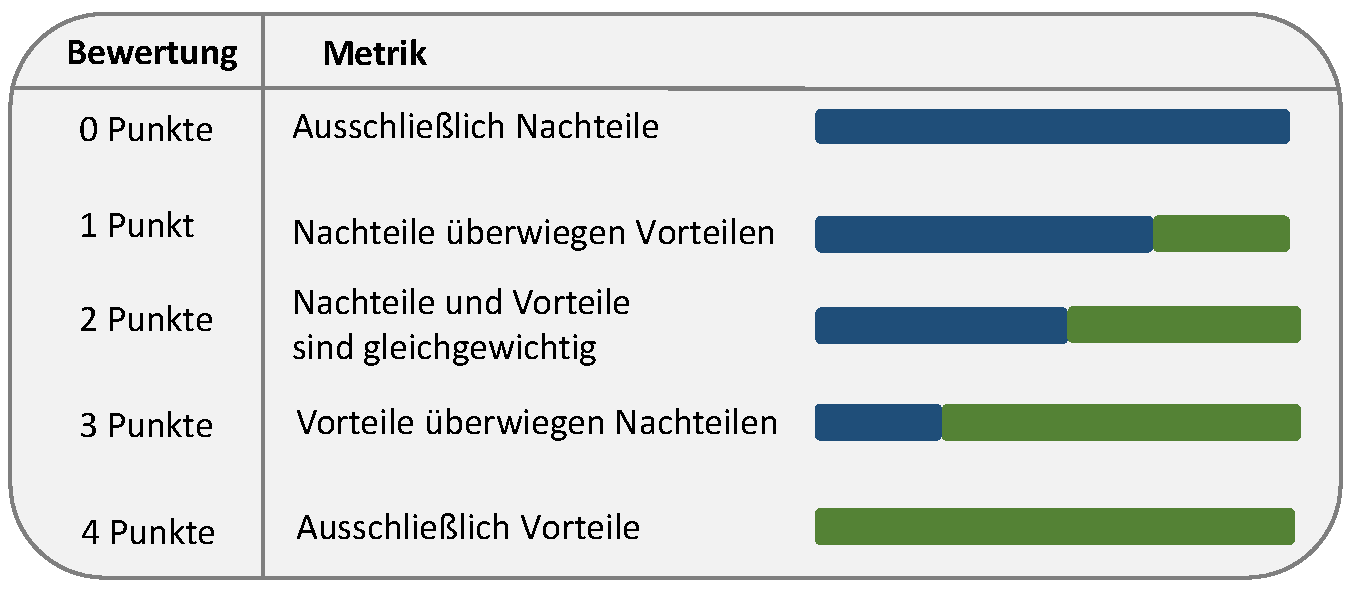
\includegraphics{Metrik}}
		\caption[Qualitative Bewertungsmetrik für AHP]{Qualitative Bewertungsmetrik für AHP. Eigene Darstellung.}
		\label{fig:metrik}
	\end{figure}
\end{center}
\vspace*{-15mm}
Aufgrund des qualitativen Evaluations-Designs wird diese Metrik für \textit{Funktionalität (K1)}, \textit{Integrationsmöglichkeiten (K2)}, \textit{Skalierbarkeit (K4)}, \textit{Flexibilität (K5)}, \textit{Administrativer Support (K7.1)}, \textit{Sicherheit (K8)} und \textit{Benutzerfreundlichkeit (K9)} angewendet. Da für die verschiedenen Pipelines divergierende Preismodelle festgelegt sind, kann für das Kriterium \textit{Kosten (K3)} ebenfalls ausschließlich eine qualitative Erörterung abgewickelt werden. Für das quantitative Kriterium \textit{Performance (K5)} wird eine divergierende Metrik definiert: 
\begin{center}
	\begin{figure}[H]
		\centering
		\scalebox{0.5}{\includegraphics{metrik_qual}}
		\caption[Quantitative Bewertungsmetrik für AHP]{Quantitative Bewertungsmetrik für AHP. Eigene Darstellung.}
		\label{fig:metrik_qual}
	\end{figure}
\end{center}
\vspace*{-15mm}
In Kriterium K7.2 (\textit{Community-Support}) wird die Anzahl der abgesetzten Blog-Posts zu einer CI/CD-Lösung untersucht. Dabei wird eine inverse Bewertung der in Abb. \ref*{fig:metrik_qual} beschriebenen Metrik durchgeführt. Dabei werden vier Punkte für die höchste Blog-Post-Anzahl vergeben. Für die restlichen Bewertungen wird invers nach dem in Abb. \ref*{fig:metrik_qual} definierten Abstufungen verfahren. Mit dieser Metrik können die relativen Kosten bzw. Blog-Posts der CI/CD-Pipelines verglichen werden. Indem der niedrigste bzw. höchste Wert als Basisgröße verwendet wird, ermöglicht sich ein Vergleich in Relation zur besten Entscheidungsalternative. Das vorliegende Bewertungs-Design erweist sich als vorteilhaft, da es ermöglicht eine Bewertung unabhängig von spezifischen Referenzwerte vorzunehmen.

\subsection{Gewichtung der Bewertungskriterien}

\subsection{Bewertung der Entscheidungsalternativen}
Das Erste zu bewertende Kriterium ist die \textbf{Funktionalität}. Sowohl für Jenkins als auch für Azure DevOps wird die Programmbibliothek Project Piper verwendet. Daher erzielen beide CI/CD-Pipelines innerhalb der \textit{Funktionalität} weitgehend ähnliche Ergebnisse.
Im Kriterium \textit{Tests} (K1.1) wird die Unterstützung von Unit-, Integration-, E2E sowie Manual-Tests untersucht. Mit der Programmbibliothek Project Piper wird eine Test-Laufzeitumgebungen für Node zur Verfügung gestellt. Somit können mit dieser sowohl Frontend- als auch Backend-Unit-Tests ausgeführt werden. Zur Automatisierung von Integration-Tests wird eine Newmann-Laufzeitumgebung für das Backend bzw. eine Webdriver.io-Laufzeitumgebung für OPA5-Frontend-Tests zur Verfügung gestellt. Da für E2E-Test mit OPA5 ebenfalls die Webdriver-Laufzeitumgebung verwendet wird, werden diese Validierungen ebenfalls durch Project Piper unterstützt. In dem SAP CI/CD-Service können alle Tests mit Ausnahme der Backend-Integration-Tests mit Newmann ausgeführt werden. CEs sind aufgrund ihrer modularen IT-Architektur darauf angewiesen, dass einzelne Microservices reibungslos miteinander interagieren. Aus diesem Grund stellt die Inkompatibilität von Integration-Tests einen Nachteil für den SAP CI/CD-Service dar. Da ein implizites Validieren des Kommponentenzusammenspiels ebenfalls über E2E-Tests abgewickelt wird, fällt dieser Nachteil jedoch weniger gewichtig aus. Aus diesem Grund wird eine Bewertung von 3 Punkten für den SAP CI/CD-Service vergeben (Vorteile überwiegen Nachteile). Für Azure DevOps sowie Jenkins ist eine Bewertung mit 4 Punkten vorgesehen (ausschließlich Vorteile). In Kriterium K1.2 erfolgt eine Validierung der durch die Pipeline bereitgestellten \textit{Code-Analyse-Funktionalitäten}. Mit dem Project Piper werden statische Codeanalyse mit Lint bzw. SonarQube, Sicherheitsüberprüfungen mit Checkmarx und DASTER sowie Performance-Tests mit Daster unterstützt. Mit dem SAP CI/CD-Tool sind ausschließlich statische Code-Analysen mit Lint bzw. SonarQube möglich. Neben der fehlenden Unterstützung von Performance-Tests birgt insbesondere die Inkompatibilität von Sicherheits-Tools  für CEA erhebliche Nachteile. Die CE-typische Verwendung von APIs zur Kommunikation zwischen einzelnen Microservices hat zur Folge, dass eine für unautorisierte Zugriffe begünstigte Angriffsfläche entsteht. Obwohl mögliche Sicherheitsbedenken auch durch Security-Experten manuell behoben werden könnten, ist dies bei der von CEs angestrebten schnellen Reaktionsfähigkeit hinderlich. Zudem wird die Abwicklung von \textit{\ac{SAST}} mit Checkmarx bzw. \textit{\ac{DAST}} mit DASTER von der SAP als Produktqualitätsstandard vorgeschrieben. Somit kann die SAP CI/CD-Pipeline nicht für interne Standardentwicklungen verwendet werden. Aus diesem Grund ergibt sich eine Bewertung von einem Punkt für den SAP CI/CD-Service (Nachteile überwiegen) und vier Punkten für Jenkins bzw. Azure DevOps (ausschließlich Vorteile). In Kriterium K1.3 wird die\textit{Build-Funktionalität} der Pipelines evaluiert. Mit Project Piper wird dabei das für SAP UI5 sowie SAP CAP benötigte MTA-Build-Tool unterstützt. Weiterhin wird durch die Programmbibliothek ein Build-Tool für Docker-Container bereitgestellt.  Die kompilierten Anwendungsprogramme können mit Project Piper in einem Artefakt-Repository bereitgestellt werden. Im SAP CI/CD-Service wir kein Docker-Workflow sowie Repository-Artefakt unterstützt. Besonders gewichtig ist dabei die fehlende Unterstützung des Artefakt-Repositories. Artefakt-Repositories spielen für CEs eine essenzielle Rolle bei der Durchführung von Rollbacks. Bei dem Auftreten von Fehlern kann zu einer im Artefakt-Repository abgelegten früheren Version zurückgekehrt werden. Somit wird das Risiko von Ausfällen und Unterbrechungen im Geschäftsbetrieb minimiert. Da der SAP CI/CD-Service dennoch das für SAP CAP und SAP UI5 benötigte MTA-Build-Tool bereitstellt und somit den minimal erforderlichen Satz an benötigter Build-Funktionalität unterstützt, wird eine Bewertung von zwei Punkten veranschlagt (Nachteile und Vorteile gleichgewichtig). Für Azure Pipelines sowie Jenkins wird eine Bewertung von 4 Punkten vergeben (Nur Vorteile). In Kriterium K1.4 erfolgt eine Evaluierung der \textit{Deploy- und Release-Funktionalitäten}. Dabei herrscht bei SAP CI/CD-Service, Azure Pipelines sowie Jenkins Feature-Parität. Mit den Pipelines wird eine Bereitstellung sowohl in die Cloud-Foundry-Laufzeitumgebung als auch in das SAP CTM unterstützt. Eine Optimierung der Bereitstellungsprozesse durch das SAP CTM wird dabei insbesondere innerhalb von komplexen ERP-Systemlandschaften erzielt. So könnte ein Unternehmen etwa Systeme für das Entwickeln (DEV), Testen (TEST) sowie für die Produktionsumgebung (PROD) besitzen. Während die Verantwortung des Entwickler dabei auf die ordnungsgemäße Bereitstellung Development-System verantwortlich ist, können nachfolgende Schritte von dem Betriebsteam über das SAP CTM verwaltet werden. Über dieses System können dabei vielfältige Release-Konfigurationen wie z.B. eine zeitplangesteuerte Bereitstellung vorgenommen werden. Zudem können über das SAP CTM Abhängigkeiten  verschiedenen Services festgelegt werden. Experte 2 bemerkt, dass dies insbesondere für CEA von hoher Bedeutung ist \cite[Z. 64]{ProductManagerSAPHyperspaceCICD.}. Im Falle einer API-Änderung bestimmter Microservices, besteht die Möglichkeit das in konsumierenden Diensten entsprechend Fehler auftreten. Mittels des SAP CTMs kann jedoch reguliert werden, dass die neue Version eines Microservices erst nach Anpassung der abhängigen Dienste in das Produktivsystem eingeführt wird (s. Abb. \ref*{fig:CTM}).
\begin{center}
	\begin{figure}[H]
		\centering
		\scalebox{0.3}{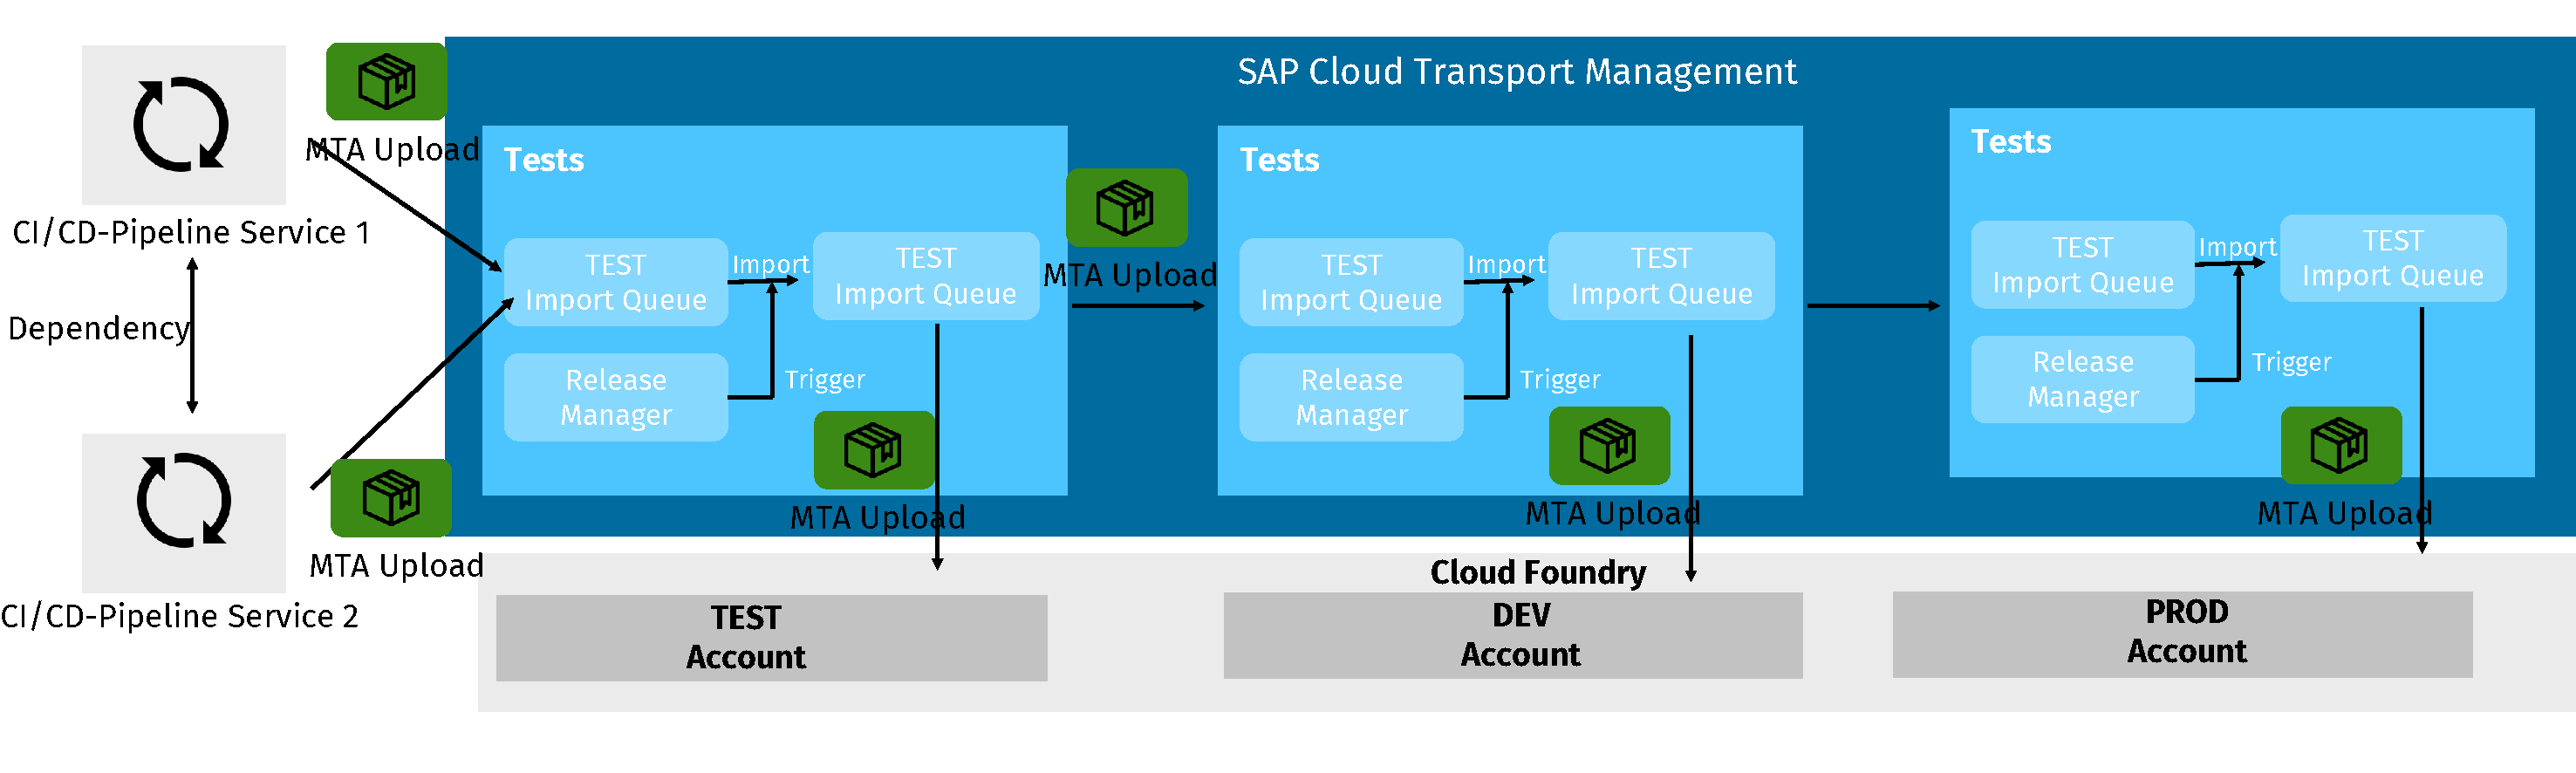
\includegraphics{CTM}}
		\caption[SAP Cloud Transportmanagement]{SAP Cloud Transportmanagement. In Anlehnung an Stevens \cite{.20230327}.}
		\label{fig:CTM}
	\end{figure}
\end{center}
\vspace*{-10mm}
Weiterhin wird von den Pipelines das Ausrollen einer neuen Anwendungsversion mit dem Blue/Green-Deployment unterstützt. Diese Strategie gewährleistet die notwendige Flexibilität und Agilität, welche es in CEs benötigt. Da im Blue-Green-Deployment neben der zu installierenden neuen Version ebenfalls die stabile Anwendung betrieben wird, können mit dieser Bereitstellungsstrategie Unterbrechungszeiten vermieden werden. Dies spielt insbesondere im Kontext von Composable-ERP-Systemen, in welchem etwa kritische Finanzprozesse abgewickelt werden, eine wichtige Rolle. Da die CI/CD-Lösungen kein Canary-, Shadow- sowie Ramped-Deployment unterstützen wird eine Bewertung von 3 Punkten abgegeben (Vorteile überwiegen). In Kriterium K1.5 wird die \textit{Monitoring-Funktionalität} der Pipelines untersucht. Mit Project Piper können im CI/CD-Prozess generierte Logs unmittelbar an das Monitoring-Dashboard Splunk übermittelt werden. Open-Soruce-Tools wie das Kibana-Dashboard lassen sich dabei ebenfalls mit Jenkins bzw. Azure Pipelines verknüpfen. Während Kibana unmittelbar als Azure-SaaS-Tool verfügbar ist, benötigt das Aufsetzen auf Jenkins einen deutlich höheren Aufwand (s. Abb. \ref{fig:kibana}). 
\begin{center}
	\begin{figure}[H]
		\centering
		\scalebox{0.3}{\includegraphics{kibana}}
		\caption[Pipeline-Monitoring mit Kibana und Jenkins]{Pipeline-Monitoring mit Kibana und Jenkins. In Anlehnung an Atta}
		\label{fig:kibana}
	\end{figure}
\end{center}
\vspace*{-15mm}
So müssen auf der Jenkins-Plattform Tools zum Versenden (Beats), Transformieren (Logstash) bzw. zum Speichern der Piepline-Logs (Elasitcsearch) manuell aufgesetzt werden. Um die Pipeline-Metriken letztlich auf dem Dashboard zu visualisieren, müssen die Logs über APIs an eine extern gehostete Kibana-Instanz übermittelt werden. Der SAP CI/CD-Service unterstützt ausschließlich ein reines Protokollieren der Build-Logs einzelner Pipelines. Die Inkompatibilität von Monitroing-Dashboards stellt dabei insbesondere für CEA einen erheblichen Nachteil dar. Für Experte 2 stellen diese zentralen Dashboards bei aus komplexen Microservices bestehenden Systemarchitekturen häufig die einzige Möglichkeit dar CI/CD-Prozesse nachhaltig zu überwachen \cite[Z. 39]{ProductManagerSAPHyperspaceCICD.}. Während für Azure Pipelines vier Punkte vergeben werden (ausschließlich Vorteile), erhält Jenkins aufgrund des hohen Einrichtungsaufwands für Kibana-Dashboard eine Bewertung von drei Punkten (Vorteile überwiegen). Für die SAP CI/CD-Pipeline wird aufgrund der fehlenden Unterstützung von Monitoring-Tools ein Punkt vergeben (Nachteile überwiegen).\\
In Kriterium K2 werden die \textbf{Integrationsmöglichkeiten} der Pipelines evaluiert. Alle drei Pipelines unterstützen dabei eine Integration der Repositories GitHub, BitBucket und GitLab (Kriterium K2.1). Für Jenkins und den SAP CI/CD-Service müssen in den entsprechenden Repositories Webhooks aufgesetzt werden. Ein Webhook ist eine HTTP-Anfrage, welche an den Dienst einer CI/CD-Pipeline gesendet wird. Sobald diese Webhook-Anfrage eintrifft, wird ein automatisiertes Auslösen des CI/CD-Workflows initiiert. Diese Webhook-Anfragen können bei einer Vielzahl von Events, einschließlich dem \textit{Pushen} von Codeänderungen oder dem Eröffnen von \textit{Pull-Requests}, ausgelöst werden. Die SAP CI/CD-Pipeline unterstützt dabei keine Pull-Request-Webhooks. Dies birgt im Entwicklungsprozess erhebliche Nachteile. Eine Pull-Request-Pipeline gewährleistet, dass Entwicklungen eines Feature-Branches erst nach erfolgreicher Abwicklung aller Tests in den Hauptzweig integriert wird. Ohne diese Funktionalität muss die Pipeline stets manuell gestartet und überprüft werden, was zur Beeinträchtigung der Zusammenarbeit in Teams führt. Mit Azure Pipelines lassen sich die untersuchten Repositories unmittelbar in die CI/CD-Tools integrieren. Somit entällt für diesen Service das manuelle Aufsetzen von Webhook-APIs sowie Authentifizierungstoken. Aus diesem Grund wird eine Bewertung von 4 Punkten für Azure Pipelines (ausschließlich Vorteile) bzw. 3 Punkten für Jenkins vergeben (Vorteile überwiegen). Da eine Pull-Request-Pipeline in einigen Entwicklungsabteilungen gängige Praxis darstellt, wird eine Bewertung von 2 Punkten vergeben (Vorteile und Nachteile gleichgewichtig). 
In Jenkins sowie Azure Pipelines lassen sich die Entwicklungsumgebungen Microsoft Visual Studio Code sowie Eclipse integrieren (Kriterium K2.2). Die SAP CI/CD-Pipeline unterstützt keine der zu evaluierenden Entwicklungsumgebungen. Somit ist es Entwicklern nicht möglich die CI-Pipeline unmittelbar aus der Entwicklungsumgebung zu starten. Somit ergibt sich eine Bewertung von drei Punkten für Azure Pipelines sowie Jenkins (Vorteile überwiegen Nachteile) bzw. null Punkte für den SAP CI/CD-Service (ausschließlich Nachteile). Sowohl mit Azure Pipelines als auch Jenkins lassen sich Planungstools wie Jira integrieren. Für den SAP BTP-Service besteht diese Integrationsmöglichkeit nicht. Demnach ist es Projektmanagern nicht möglich den Build-Status verschiedener Backlog-Items zu begutachten. Aus diesem Grund ergibt sich eine Bewertung von vier Punkten für Azure Pipelines sowie Jenkins  bzw. null Punkte für den SAP BTP-Service.\\
In Kriterium K3 werden die \textbf{Kosten} der CI/CD-Pipelines evaluiert. Für den SAP CI/CD-Service werden Gebühren von einem Euro pro Build-Stunde fällig. Azure Pipelines berechnet hingegen unabhängig von der Nutzungszeit 40 Euro pro Pipeline. Sowohl für Azure Pipelines als auch für den SAP BTP Service werden für Kunden Rabatte vergeben. Da dies jedoch unternehmens- bzw. situationsabhängig ist, kann dieser Aspekt in der Bewertung nicht berücksichtigt werden. In die genannten Preise der beiden Anbieter werden Kosten für die IT-Infrastruktur, Installation, Wartung sowie Support einberechnet. Zwar fallen für die Jenkins-Pipeline keine Lizenzgebühren an, jedoch müssen im Gegensatz zu den SaaS-Pipelines weitere TCO-Positionen beachtet werden. Da Jenkins von den Unternehmen selbst bereitgestellt werden, müssen hierbei zunächst Investitionskosten für Hardware berücksichtigt werden. Darüber hinaus fallen ebenfalls Personalaufwendungen für Sicherung der Plattformdaten, Überwachung der Systemleistung sowie das Einspielen von Updates an. Die hohen Investitionskosten sorgen dafür, dass On-Premise insbesondere in einer kurzfristigen Betrachtung teurer ist. Dies gilt jedoch nur unter der Annahme, dass keine Veränderungen an der IT-Infrastrukur vorgenommen werden. CEs sind jedoch darauf ausgerichtet flexibel und agil zu agieren, um auf sich ändernde Geschäftsanforderungen reagieren zu können. Somit müssen diese in der Lage sein, Systeme schnell auf- und abzubauen. Dies würde im On-Premise-Modell sehr hohe Investitionskosten verursachen, wobei das SaaS auch auf längere Sicht die günstigere Alternative bleibt. Aus diesem Grund wird für die SaaS-Systeme Azure Pipelines und SAP CI/CD eine Bewertung von drei Punkten bzw. für Jenkins zwei Punkten vergeben (Nachteile und Vorteile gleichgewichtig).\\
In Kriterium K4 wird die \textbf{Skalierbarkeit} der Pipelines evaluiert. Mit Azure Pipelines lässt sich die CI/CD-Pipeline eines Microservices horizontal skalieren. Um parallele Builds auszuführen, werden hierbei mehrere \textit{Microsoft-hosted Agents} aktiviert. Ein Microsoft-hosted Agent ist eine von Azure gehostete virtuelle Maschine, welche eine vorkonfigurierte Build- und Testumgebung bereitstellt. Eine vertikale Skalierung kann dabei durch das Zuweisen zusätzlicher Ressourcen zu einem Microsoft-hosted Agent erreicht werden. Mit Jenkins ist ebenfalls eine horizontale Skalierung möglich. Dafür muss den sog. \textit{Jenkins-Agents} jedoch eine separate virtuelle Maschine oder sogar ein eigenes System bereitgestellt werden. Eine vertikale Skalierung ist aufgrund architektonischer Einschränkungen nur begrenzt möglich. So müssen in das bestehende System zusätzliche Hardware-Ressourcen integriert werden. Somit ist die vertikale Skalierbarkeit auf die physische Einschränkung des Servers begrenzt. Sowohl horizontale als auch vertikale Skalierung ist mit dem SAP CI/CD-Service nicht realisierbar. Dabei spielt die Skalierbarkeit von CI/CD-Pipelines insbesondere in einem volatilen Geschäftsumfeld eine signifikante Rolle. Als eines der größten Composable-Enterprises stellt der Streaminganbietern Netflix über 700 Microservices bereit. Da für jeden Microservices mindestens eine CI/CD-Pipeline benötigt wird, erfordert die  Bereitstellung der Dienste eine umfangreiche IT-Infrastruktur. Netflix setzt dabei auf eine skalierbare Container-Orchestrierungstechnologie. Eine effiziente Nutzung von Ressourcen kann somit durch das automatische Erstellen von Containern bei Auslösung eines CI/CD-Builds und deren anschließende Löschung nach Abschluss eines Jobs erreicht werden. So wird Azure Pipelines mit vier Punkten, Jenkins mit drei Punkten und der SAP CI/CD-Service mit null Punkten bewertet.\\ 
In Kriterien K6 wird die \textbf{Flexibilität} der Services evaluiert. Sowohl mit Azure als auch Jenkins lassen sich die mit der Programmbibliothek Project Piper bereitgestellten CI/CD-Schritte (z.B. Build, Test etc.) frei nach Bedarf kombinieren und zu konfigurieren. Der SAP CI/CD-Service unterliegt dabei maßgeblicher Einschränkungen. Hierbei werden Anzahl, Reihenfolge sowie Konfiguration der Schritte von dem Service vorgeschrieben. Somit ist keine flexible Implementierung der Pipelines möglich. Wie von Experte 5 hervorgegangenen, stellt Technologieoffenheit einen fundamentalen Wert der CEA dar \cite[Z. 10]{SoftwareArchitektSAPDTSIntegration.}. So sollte die CI/CD-Pipeline in der Lage sein verschiedene Programmierframeworks, Test-Tools und Cloud-Plattformen zu unterstützen. Dafür wird in Jenkins eine Bibliothek mit mehr als 1500 Plug-ins bereitgestellt, womit Funktionalitäten, welche über den Standard hinausgehen, integriert werden können. Während mit Azure Pipelines 200 Plug-ins bereitgestellt werden besteht diese Möglichkeit im SAP CI/CD-Service nicht. Um schnell neue Microservices bereitzustellen, sollte die CI/CD-Pipeline eines CEs einen modularen Aufbau ermöglichen. Für Azure Pipelines und Jenkins wird durch die Verwendung von Project Piper das Shared-Library-Konzept realisiert (s. Abb. \ref{fig:Modular}). Damit ist es möglich ausgewählte Funktionalitäten oder Prozesse in einer gemeinsamen Bibliothek zu konsolidieren. Mit Project Piper werden standardisierte CI/CD-Schritte zu Versionierungs-, Build-, Test-, Security-Schritten etc. bereitgestellt. Eine weitere Möglichkeit um die Komplexität der Bereitstellung zu reduzieren, besteht in der Wiederverwendung ganzer Pipelines. Die zugrundeliegende Konzeption besteht darin, dass sämtliche Microservices einen homogenen Bereitstellungszyklus durchlaufen. Somit werden diese auf analoge Weise kompiliert, verpackt und bereitgestellt. Demnach kann eine Pipeline für verschiedene Microservices wiederverwendet werden. Bei Jenkins und Azure lässt sich dies durch die Einbindung mehrerer Repositories in eine Pipeline realisieren. Im SAP CI/CD-Service wird ebenfalls ein Shared-Library-Konzept unterstützen. So werden die templatebasierten Schritte ebenfalls als standardisierte Elemente einer CI/CD-Pipeline ausgeliefert. Die Wiederverwendung ganzer Pipelines für unterschiedliche CI/CD-Services ist hingegen nicht möglich.
\begin{center}
	\begin{figure}[H]
		\centering
		\scalebox{0.6}{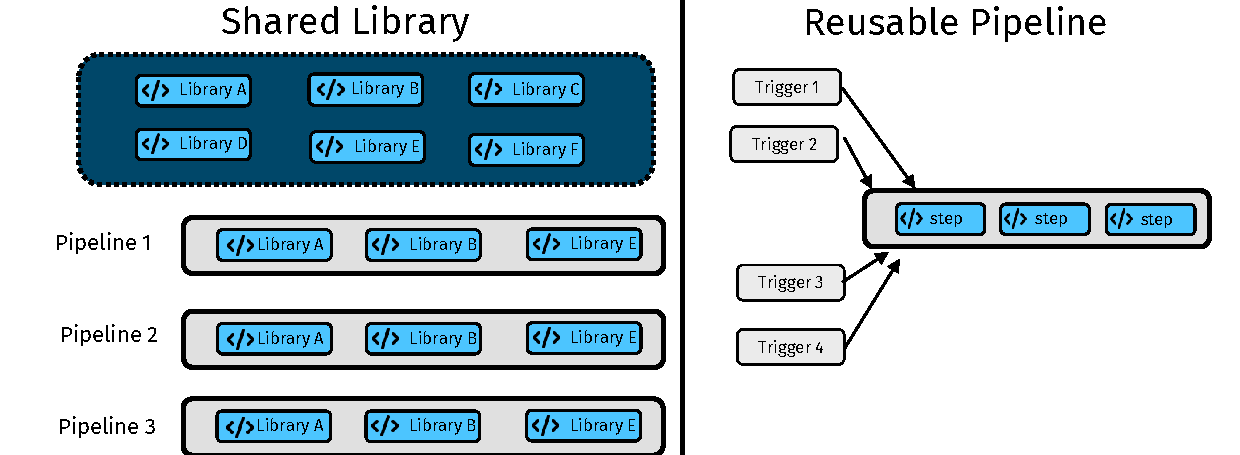
\includegraphics{Modular}}
		\caption[Modularer Aufbau einer CI/CD-Pipeline]{Modularer Aufbau einer CI/CD-Pipeline. In Anlehnung an Codefresh \cite{.20230402}.}
		\label{fig:Modular}
	\end{figure}
\end{center}
\vspace*{-15mm}
Während der SAP CI/CD-Service das Shared-Library-Konzept unterstützt, ist eine flexible Implementierung der Pipelines, die Einbindung von Plug-ins, sowie die Wiederverwendung von CI/CD-Pipelines nicht möglich. Deshalb wird für den SAP CI/CD-Service eine Bewertung von einem Punkt vergeben (Nachteile überwiegen Vorteile). Da Jenkins und Azure Pipelines bei den zu untersuchenden Entscheidungskriterien nur Vorteile bieten, werden jeweils vier Punkte vergeben.\\
In Kriterium K8 wird der \textbf{Support} der CI/CD-Pipelines evaluiert. Azure Pipelines stellt  einen umfangreichen \textit{administrativer Support} bereit (Kriterium K7.1). So besteht für Kunden die Möglichkeit einen Premium-Support in Anspruch zu nehmen. Dabei handelt es sich um eine kostenpflichtige Leistung, welche den Kunden unmittelbaren Zugang zu technischem Support und Beratung gewährt. Die Unterstützung beinhaltet Installation bzw. Konfiguration von Pipelines, Integration einer vorhanden CI/CD-Toolchain (Tests, Repositories etc.) einschließlich der Optimierung der Pipeline-Performance. Zudem wird über den Azure-Support-Center ein kostenfreies Support-Ticket-System angeboten. Für Kunden besteht die Möglichkeit diese Kanäle zu nutzen, um allgemeine technische Probleme des CI/CD-Services zu melden. Weiterhin wird von Azure eine umfangreiche Dokumentation sowie Schulungsmaterialien, einschließlich Online-Tutorials, Videos und Webinare bereitgestellt. Beim SAP CI/CD-Service wird Kundenservice über Service Now bereitgestellt. Service Now ist ein führender Anbieter für IT-Service-Management-Lösungen. Dieser Dienst ermöglicht die Erstellung von Tickets bei technischen Problemen. Bei spezifischen Fragestellungen zum CI/CD-Service erhalten die Kunden technische Unterstützung durch Berater der SAP. Wie auch bei Azure Pipelines stehen Schulungs- und Dokumentationsunterlagen für den SAP CI/CD-Service zur Verfügung. Für Jenkins sind diese Informationsmaterialien ebenfalls vorhanden, jedoch ist der administrative Support aufgrund des Open-Source-Charakters im Vergleich zu den andere Lösungen begrenzt. Dies ist insbesondere auf das Fehlen eines unmittelbaren Supports durch einen Service-Anbieter zurückzuführen. Ebenso spiegelt sich dieser Aspekt in der Verfügbarkeit von Updates wider. Viele Funktionalitäten von Jenkins werden über Open-Source-Plug-ins bereitgestellt. Experte 6 merkt an, das dabei jedoch immer das Risiko besteht, dass die Wartung einzelner Plug-ins in Zukunft vernachlässigt werden könnte \cite[Z.30]{FullStackEntwicklerSAPDTSIntegration.}. Aus den hier aufgeführten Aspekten ergibt sich eine Bewertung von vier Punkten für Azure Pipelines sowie dem SAP CI/CD-Service (ausschließlich Vorteile). Für Jenkins wird eine Bewertung von einem Punkt vergeben (Nachteile überwiegen). Aufgrund des Open-Source-Charakters ist für die Jenkins-Pipeline ein umfassender \textit{Community-Support} vorhanden (Kriterium K7.2). Jenkins ist dabei auf zahlreichen hochfrequentierten Foren vertreten. So wurden auf Stackoverflow bereits 112000 Posts zur Jenkins-Pipeline veröffentlicht \cite{StackOverflow.20230403d}. Dies bietet Anwendern den Zugriff auf eine breite Palette an Ressourcen, um Fragen und Probleme lösen zu können. Dabei merkt Experte 4 an, dass insbesondere die Gamifizierung dieser Plattformen zu einer schnellen und effektiven Unterstützung durch Spezialisten beitragen. Auch Azure Pipelines sowie der SAP CI/CD-Service sind ebenfalls auf öffentlichen Community-Foren vertreten, jedoch ist der dort publizierte Inhalt im Vergleich zu Jenkins signifikant geringer. Das liegt an der Tatsache, dass die genannten Pipelines als SaaS-Lösungen konzipiert sind und somit weniger Raum für fragebedürftige Anpassungen bestehen. So sind für Azure Pipelines 25000 Post und für den SAP CI/CD-Service lediglich 26 Einträge auf Stackoverflow veröffentlicht \cite{StackOverflow.20230403b}\cite{StackOverflow.20230403c}. Gemäß der in Kapitel \ref{sec:Metriken} festgelegten Metrik erzielt wird eine Bewertung von vier Punkten für Jenkins (höchste Blog-Post-Anzahl) bzw. von einem Punkt für Azure Pipelines und dem SAP CI/CD-Service vergeben (0 Prozent bis 25 Prozent unter dem höchsten Wert).\\
In Kriterium K8 wird die \textbf{Sicherheit} der CI/CD-Tools evaluiert. Jenkins bietet flexible Möglichkeiten zur Authentifizierung. Neben einer integrierten Benutzerverwaltung lassen sich über Jenkins auch Drittanbieterdienste wie Github, Google, BitBucket oder SAP-\acl{SSO} (SAP-\acs{SSO}) einbinden. Bei Jenkins ist ebenfalls die Implementierung eines Rollenkonzeptes möglich. Dabei können Rollen und Berechtigungen erstellt, welche bestimmten Benutzer zugewiesen werden. Damit kann sichergestellt werden, dass kritische Konfiguration ausschließlich von Spezialisten vorgenommen werden. Für Azure Pipelines sowie dem SAP CI/CD-Service werden ebenfalls Authentifizierungsmöglichkeiten unterstützt. Die Implementierung eines Rollenkonzeptes ist im SAP CI/CD-Service jedoch nicht möglich. Aufgrund der Integration eines Plug-in-Ökosystems bietet die Jenkins-Pipeline im Kontext der Systemsicherheit ein erhöhtes Risiko von unbefugten Zugriffen. Da in einer Community für jeden Entwickler die Möglichkeit besteht, Plug-ins zu veröffentlichen, besteht die Möglichkeit, dass Sicherheitsrisiken vor der Installation nicht ausreichend überprüft werden. Wie von Experte 5 angemerkt besteht dabei das Risiko, dass feindliche Programe in den Build-Prozess des CI/CD-Workflows eingeschleust werden, welche wiederum negative Auswirkungen auf das Produktivsystem besitzen \cite[Z. 39]{SoftwareArchitektSAPDTSIntegration.}. Auch bei Azure Pipelines ist die Einbindung von Plug-ins möglich. Da hierbei jedoch ausschließlich validierte auf dem Azure Marketplace bereitgestellte Plug-ins integrierbar sind, fällt das korrespondierende Sicherheitsrisiko deutlich geringer aus. Da IT-Sicherheit zum Kerngeschäft von Cloud-Providern wie Microsoft oder SAP gehört, verfügen diese über erfahrenes Sicherheitspersonal, welches ein tiefes Verständnis über aktuelle Bedrohungen und Angriffsmethoden verfügt. Somit lässt sich schlussfolgern, dass sowohl Azure Pipelines als auch der SAP CI/CD-Service ein hohes Niveau an Systemsicherheit bieten. Ein Vorteil der On-Premise-Bereitstellung mit Jenkins ist, dass Unternehmen vollständige Kontrolle über die Systemkonfiguration behalten. Dieser Aspekt ergibt sich ebenfalls im Hinblick auf die Ausfallsicherheit. Betreibt ein Unternehmen CI/CD-Pipelines auf firmeneigenen Servern, ist es diesem möglich, gezielte Maßnahmen zur Verbesserung der Ausfallsicherheit zu ergreifen. Im Gegensatz dazu hängt die Verfügbarkeit der SAP CI/CD-Lösung bzw. von Azure Pipelines in erheblichem Maße von den Cloud-Anbietern ab. Azure und SAP legen vertraglich jedoch eine Verfügbarkeit von  99,9 bzw. 99,5 Prozent fest. Aufgrund der situativen Gegenheiten werden Vor- und Nachteile der On-Premise- bzw. Cloud-Bereitstellung als gleichwertig betrachtet. Daraus resultiert sowohl für Azure Pipelines als auch für den SAP CI/CD-Service eine Bewertung von zwei Punkten. Aufgrund der zusätzlichen Sicherheitsrisiken im Zusammenhang mit dem Plug-in-Ökosystem wird für Jenkins eine Bewertung von einem Punkt vergeben (Nachteile überwiegen Vorteile). In Kriterium K9 wird die Benutzerfreundlichkeit der Pipelines evaluiert. Da Azure Pipelines und der SAP CI/CD-Service als SaaS vertrieben werden, bieten diese hinsichtlich der \textit{Installation und Wartung (Kriterium K2)} einige Vorteile. Da es sich hierbei um cloudbasierte Lösungen handelt, entfällt die Notwendigkeit CI/CD-Tools in einem lokalen Rechenzentrum zu installieren. Auch die Wartung der IT-Infrastruktur liegt in Verantwortung der Cloud-Anbieter. Dadurch werden IT-Spezialisten zeitlich entlasten, wodurch IT-Fachpersonal verstärkt auf die Kernkompetenzen des Unternehmens fokussiert werden können. Da Jenkins in einer On-Premise-Umgebung betrieben wird, obliegt die Verantwortung der Installation und Wartung bei den Unternehmen selbst. Daraus resultiert eine Bewertung von vier Punkten für Azure Pipelines und dem SAP CI/CD-Service (ausschließlich Vorteile) bzw. von null Punkten für Jenkins (ausschließlich Nachteile). Azure Pipelines und der SAP CI/CD-Service bieten im Hinblick auf die \textit{intuitive Bedienbarkeit} eine webbasierte Benutzeroberfläche, über welche Builds-Prozesse, Systemkonfigurationen und Pipelines eingesehen und angepasst werden können. Die Implementierung der Pipeline erfolgt dabei jedoch über Code. Während für Azure Pipelines eine YAML-Syntax verwendet wird, werden CI/CD-Pipelines in Jenkins über Groovy implementiert. Unter Verwendung von Project Piper kann eine Pipeline jedoch mit minimalem Aufwand an Code erstellt werden. Im Gegensatz dazu benötigt der SAP CI/CD-Service überhaupt keine manuelle Implementierung über Code. So können die Anwender mithilfe einer webbasierten Benutzeroberfläche die gesamte Implementierung einer Pipeline konfigurieren. Dies ist dabei insbesondere für CEs von wesentlicher Bedeutung. Bei der Bereitstellung neuer Microservices ist ggf. die Implementierung einer neuen Pipeline erforderlich. Eine intuitive Bedienbarkeit bietet dabei erhebliche Vorteile, um bei der Erstellung von Pipelines Zeit zu sparen. Aus diesem Grund erhält der SAP CI/CD-Service eine Bewertung von vier Punkten (ausschließlich Vorteile). Obwohl Project Piper grundsätzlich zur Vereinfachung der Implementierung beitragen kann, benötigt es einer aufwändigen Programmierung von Anforderungen, welche über den Bibliotheksstandard hinausgehen. Aus diesem Grund wird für Azure Pipelines sowie dem SAP CI/CD-Service eine Bewertung von einem Punkt vergeben (Nachteile überwiegen).

\subsection{Entwicklung einer ganzheitlichen Bereitstellungsstrategie}
 
